% NOTES:
%
% . Search for TODOs in the text for issues that need to be
%   resolved.
%
% . This is currently in a book format.  This format makes sense for an overview
%   document, but if we prepare a journal article we'll need to switch to an article
%   format.
%

% TODO: should we stick with LaTeX documentation?  It might make sense
% to migrate to reStructured text, since that is a Python standard and
% since it can generate LaTeX.  We'll have to decide that sometime soon.

\documentclass[12pt]{article}

\usepackage{fullpage}
%\usepackage{secdot}
\usepackage[authoryear]{natbib}
\usepackage{listings}
\usepackage{url}
\usepackage[usenames]{color}

\bibpunct{[}{]}{,}{n}{}{}

\usepackage{graphicx}
%%\usepackage{helvet}
%%\usepackage{courier}
%%\usepackage{makeidx}
%%\usepackage{multicol}
%%\usepackage{mathptmx}
%%%\usepackage{type1cm}
%%%\usepackage[bottom]{footmisc}
%%%\usepackage{footmisc}
%%%\usepackage{amsfonts,amsmath,graphicx,subfigure}

\newcommand{\HLine}{$\mbox{ }$\hrulefill$\mbox{ }$}

\newtheorem{Rem}{Remark}

\def\Argmax{\mathop{\rm argmax}}
\def\Argmin{\mathop{\rm argmin}}

\def\Abs{\mathop{\rm abs}}
\newcommand{\Gets}{:=}

\newcommand\eg{e.g.\ }
\newcommand\ie{i.e.\ }

\newcommand{\code}[1]{\textmd{\texttt{#1}}}

\if 0
\lstinputlisting{source_filename.py}
\fi

\def\pca{PCA}
\def\pcasp{PCA\ }
\newcommand{\todo}[1]{\textbf{\textit{TODO: #1}}}




\begin{document}

\title{The PyUtilib Component Architecture}

\author{William E.\ Hart\footnote{Sandia National Laboratories, 
Discrete Math and Complex Systems Department, 
PO Box 5800, Albuquerque, NM 87185;
{\tt wehart@sandia.gov}}
\and
John Siirola\footnote{Sandia National Laboratories,
Exploratory Simulation Technologies Department, 
PO Box 5800, Albuquerque, NM 87185;
{\tt jdsiiro@sandia.gov}}
}

\date{\today}

\maketitle

\begin{abstract}
We describe the PyUtilib Component Architecture (\pca), which has
been substantially revised for the PyUtilib 4.0 release. The design
of \pcasp is inspired by the Trac component architecture, and it
supports advanced features like non-singleton components, namespaces
and caching of component interactions. The \pcasp includes an
independent, self-contained framework core that can be easily
integrated into other applications, as well as a variety of extension
packages with commonly used components.
\end{abstract}


\lstset{language=Python}
\definecolor{light-gray}{gray}{0.9}
\lstset{backgroundcolor=\color{light-gray}}
\lstset{aboveskip=1em,belowskip=1em,showspaces=false,showstringspaces=false}

\newpage
\tableofcontents
\newpage

% TODO: should we refer to 'PCA' or 'the PCA' in the text?

\section{Introduction}

Component Based Software Engineering (CBSE) has become one of the
leading approaches to developing complex extensible software
systems~\cite{HeiCou01}.  CBSE implementations frequently rely on
concepts from both object oriented programming (OOP) and event-driven
programming.  Unlike traditional OOP where classes and polymorphism
are used to manage related data-driven objects, CBSE leverages
classes and polymorphism to represent related functional interfaces
and programmatic \emph{services}.  The central idea underlying CBSE
is \emph{equivalence of service}; that is, the separation of the
declaration of component interfaces from their implementation.  This
allows for more flexible software design that encourages modularity
of component interface and definitions.  Furthermore, this segregation
allows for explicit management of the interactions among components.
We can begin to imagine software components as commodities that can
be integrated into applications in a much more flexible and dynamic
manner.

A variety of mature, general purpose environments exist
for defining and managing components (e.g., the CORBA Component
Model~\cite{CORBA_CMS} and the Common Component
Architecture~\cite{cca}).  Although 
Python interfaces have been developed for some of these environments, a
variety of native Python component environments have also been developed,
including Zope~\cite{Zope}, Envisage~\cite{Envisage}, Trac~\cite{Trac},
yapsy~\cite{yapsy} and SprinklesPy~\cite{SprinklesPy}.

This report describes the PyUtilib Component Architecture (\pca),
which was significantly revised in the PyUtilib 4.0 release.  The
\pcasp is derived from the Trac component framework~\cite{Trac},
and it is included in the PyUtilib software package~\cite{PyUtilib}.
Our development of the \pcasp was motivated by our experience with
a variety of scientific computing applications, which led to the
following requirements for \pca:
\begin{itemize}

\item \textit{Independent, self-contained framework core}: Many
  component architectures 
are embedded in larger software frameworks (e.g. Zope, Trac), which
  make it difficult 
to extract and use just the software packages related to the component
architecture.  
%\todo{Reference websites that discuss components in zope and twisted, which are the two most widely-used Python architectures.  Discuss our experience using Trac's architecture.}

\item \textit{Non-Singleton components}:  The computational science
applications that motivate \pcasp require both singleton components
(which have a single unique instance) and non-singleton components
(which have many unique instances). 

\item \textit{Namespaces}:  Using components in large software projects
requires management across multiple libraries.  Namespaces are needed
to effectively manage components in these complex software projects.

\item \textit{Caching}:  Components need to support applications
where component interfaces are called thousands or millions of times.
Thus, caching of this 
interaction 
is needed to minimize the overhead of the component architecture.

\item \textit{Loading from EGGs}:  Support for loading EGG files is
invaluable in dynamic applications.  Further, loading components from EGG
files provides another level of modularity to the management of software
applications.

\end{itemize}

A key guiding principle behind our development of the \pcasp is a focus on
simplicity and flexibility.  Our goal is to minimize the burden placed
on application developers for both adding the \pcasp to a project and
maintaining \pca-based applications.  One consequence is that the \pcasp
explicitly does not provide some advanced capabilities, like interface
validation and interface adaption, that are available in more
heavyweight component architectures such as Zope or Envisage.

%Another motivation for the development of the \pcasp was the desire to
%employ a light-weight 
%framework that could be easily deployed.  Thus, dependencies on a
%general purpose  
%environment was undesirable.  Additionally, support for interface
%conversion was not  
%deemed sufficiently important to justify the use of a more complex
%framework like Zope or 
%Envisage that supports this functionality.


\if 0

Pyomo leverages the PyUtilib Component Architecture (\pca) to support
plugins that extend Pyomo's built-in functionality.  \pcasp supports an
object oriented approach to software design, which is an accepted strategy
for managing software complexity in large systems.  Object oriented
design is traditionally done using classes and class inheritance;  classes
define interfaces, which are extended and customized in subclasses using
class inheritance.

The main idea behind \pcasp is to separate the declaration of component
interfaces from their implementation.  This allows for a more flexible
design of software components that further encourages modularity of
components.  Additionally, \pcasp includes a global component registry, as
well as a framework for automating the execution of components that match
a given interface.  This capability facilitates the dynamic registration
and application of components within large software systems.

The plugin components supported by Pyomo have a variety of significant impacts
on the development and deployment of Pyomo applications:
\begin{itemize}

\item Plugins facilitate extensions of Pyomo without risk of destabilizing core functionality.  

\item Plugins allow third-party developers to add value without requiring direct involvement of the core developers.  For example, Pyomo extensions can be developed and distributed without requiring developer access to Pyomo's subversion repository.  Similarly, third-party developers can develop 
plugins that are specific to their working environment or business needs.

\item The \pcasp can automate the activation of external software interfaces, based on the user's environment.  For example, optimization solvers can be
automatically registered if they are found with the user's \code{PATH} environment.

\item New capabilities can be dynamically loaded at run-time.  Python EGG files provide a standard, modular mechanism for distributing plugins.  The \pcasp can dynamically load EGG files, which allows users to dynamically activate 
plugins.

\end{itemize}

\fi


The remainder of this manuscript is divided into the following sections.
Section~\ref{chap:pca} provides a tutorial introduction to the use of \pcasp classes,
and Section~\ref{chap:core} provides a detailed description of \pcasp capabilities.
Section~\ref{chap:extensions} describes PyUtilib extension
packages that support specific components based on the \pca.  This section
motivates these packages and provides examples of their use.  Section~\ref{chap:disc}
discusses how the \pcasp has 
fundamentally influenced the design of the Pyomo software project.



% LocalWords:  CBSE CORBA Zope Trac yapsy SprinklesPy PyUtilib Trac's EGGs
% LocalWords:  Namespaces Pyomo plugins Pyomo's plugin Pyomo

\lstset{frame=single,
  basicstyle=\footnotesize ,
  backgroundcolor=\color{white},
  language=Python}

\section{The PyUtilib Component Architecture}

\label{chap:pca}

The PyUtilib Component Architecture (\pca) is included in the
PyUtilib software package~\cite{PyUtilib}.  It inspired by the Trac
plugin framework~\cite{Trac}, and it was initially motivated by our
need for an independent, self-contained plugin framework for
scientific computing applications.  The core of the \pcasp is
provided through a small set of classes within PyUtilib's
\code{pyutilib.component.core} package.  This section provides a
tutorial introduction of the \pcasp as well as a detailed description
of the \pcasp classes and their functionality.


\subsection{\pcasp Definitions}

There are different notions of software components~\cite{Mar05}, so we begin by
providing some definitions.  The relationships among these terms is
illustrated in Figure \ref{fig:defs}.  A \textit{plugin} is a
class that implements a set of related methods in the context of an
application.  Thus, a plugin can be described as a component definition.

An \textit{interface} class defines a type that a plugin uses to register
its capabilities.  A plugin class includes declarations that denote that
it implements one-or-more interfaces. An interface is defined by the
methods and data that are used.  However, the \pcasp does not enforce
this interface or support interface conversions (see Zope~\cite{Zope}
and Envisage~\cite{Envisage} for examples of plugin frameworks that
support this functionality).

A \textit{service} is an instance of a plugin class that is registered
globally with its interfaces.  We say that a plugin class instance
is \textit{active} if it is registered, and a plugin class instance
is only treated as a service if it is active.  A service can be an
instance of either a singleton or non-singleton plugin. There is
exactly one service for a singleton plugin (and that service is
instantiated automatically), whereas there can be multiple services
of non-singleton plugins.  Singleton plugins are active by default,
whereas non-singleton plugins are conditionally active depending
how the plugin interface is declared.

\begin{figure}[htb]
  \center
  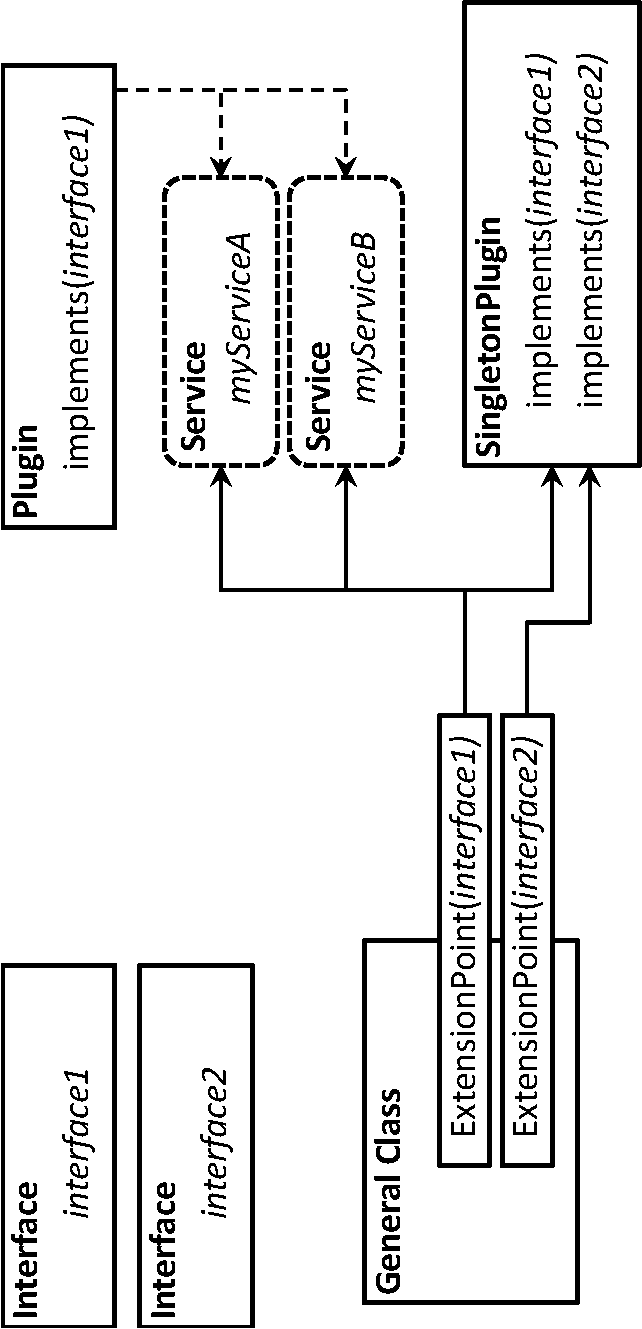
\includegraphics[height=5in,angle=-90]{figures/definitions.pdf}
  \caption{An illustration of how classes within the PCA relate to one another.  Interface classes are independent declarations of APIs.  Plugin classes can declare that they implement an Interface's API, and extension points declare that they require a specific
Interface API.  Both singleton and non-singleton plugins can be used, but services for non-singleton plugins are explicitly constructed.}
  \label{fig:defs}
\end{figure}

A software application or a component can declare \textit{extension
points} that other components can \textit{plug in} to. An extension
point is defined with respect to a specific \textit{interface}
class.  Thus, a service that supports an interface plugs into an
extension point for that interface.  In this way, extension points
provide a generic mechanism for applications to employ the functionality
provided by other services.

This mechanisms supports a flexible,
modular programming paradigm that enables software applications to
be extended in a dynamic manner.  The \pcasp includes a global component
registry and a framework for automating the execution of plugin
services.  All plugins and interfaces automatically register themselves
with the registry.  This registry then acts as a broker, dynamically providing
extension points with the appropriate matching services at run time.  
Thus, an application
developer can define extension points without knowing how they will be
implemented, and plugin developers can register extensions without
needing to know the details of how -- or where -- they are employed.
This capability facilitates the dynamic registration
and application of components within large software systems.

\subsubsection{Relationship to the Trac Component System}

The general design of \pcasp is inspired by the plugin system
included in Trac~\cite{Trac}. The \pcasp generalizes the Trac
component architecture by supporting namespace management of plugins,
non-singleton plugins, support for non-active plugin instances and
caching of interface interactions. For those familiar with Trac,
the following classes roughly correspond with each other:
\begin{center}
\begin{tabular}{|l|l|} \hline
    Trac Class Name &   PyUtilib Class Name \\ \hline
    Interface   & Interface \\
    ExtensionPoint  & ExtensionPoint \\
    Component   & SingletonPlugin \\
    ComponentManager    & PluginEnvironment \\ \hline
\end{tabular}
\end{center}
The \code{PluginEnvironment} class is used to manage plugins, but unlike Trac this class does not   need to be explicitly constructed.


\subsection{A Simple Example}

Figure~\ref{fig:example1} provides a simple example that is adapted from
the description of the Trac component architecture~\cite{TCA}. This
example illustrates the three main steps to setting up a plugin: 
\begin{enumerate}
\item Defining an interface
\item Declaring extension points
\item Defining classes that implement the interface. 
\end{enumerate}
This example begins by defining \code{ITaskObserver}, a subclass of \code{Interface}. 
Although it is not required to define methods in an interface, these
declarations provide documentation for plugin developers.
We then declare a \code{TaskList} that manages a
dictionary of tasks and descriptions.  The \code{TaskList} creates an
\code{ITaskObserver} extension point, and when a task is added to the
task list, it calls all services that implement the \code{ITaskObserver}
interface.  Finally, we define a \code{TaskPrinter} as a singleton
plugin.  The \code{TaskPrinter} implements the \code{ITaskObserver}
interface, and when called prints the task name and description.  As the
\code{TaskPrinter} is a singleton plugin, the \pcasp automatically
instantiates and registers a single \code{TaskPrinter} service.

%In this example, a singleton plugin is declared, which automatically
%registers the single component service. Non-singleton plugin services need to
%explicitly created, but they are also automatically registered. 


Assuming the module in Figure~\ref{fig:example1} 
is saved as \code{task.py}, then the following Python script 
illustrates how this plugin is used:
\begin{quotation}
\begin{lstlisting}
from task import *

# Construct a TaskList object and then add several tasks.
task_list = TaskList()
task_list.add('Make coffee', 'Need to make some coffee')
task_list.add('Bug triage', 'Double-check all issues')
\end{lstlisting}
\end{quotation}
This script generates the following output:
\begin{quotation}
\begin{lstlisting}
Task: Make coffee
      Need to make some coffee
Task: Bug triage
      Double-check all issues
\end{lstlisting}
\end{quotation}


\begin{figure}
\center
\begin{quotation}
\begin{lstlisting}
# A simple example that manages a task list.  An observer 
# interface adds actions that occur when a task is added.
from pyutilib.component.core import *

# An interface class that defines the API for plugins that
# observe when a task is added.
class ITaskObserver(Interface):

    def task_added(name, description):
        """Called when a task is added."""

# The task list application, which declares an extension point
# for observers.  Observers are notified when a new task
# is added to the task list.
class TaskList(object):
    observers = ExtensionPoint(ITaskObserver)

    def __init__(self):
        """The TaskList constructor, which initializes the list"""
        self.tasks = {}

    def add(self, name, description):
        """Add a task, and notify the observers"""
        self.tasks[name] = description
        for observer in self.observers:
            observer.task_added(name, description)

# A plugin that prints information about tasks when they
# are added.
class TaskPrinter(SingletonPlugin):
    implements(ITaskObserver)

    def task_added(self, name, description):
        print 'Task:', name
        print '     ', description
\end{lstlisting}
\end{quotation}
\caption{A simple example of \pcasp components.}
\label{fig:example1}
\end{figure}



\section{PCA Classes}
\label{chap:core}

The \pcasp consists of the following core classes that are defined in the \code{pyutilib.component.core} package:
\begin{description}
\item[Interface] Subclasses of this class declare plugin interfaces that are registered in the \pca. 
\item[ExtensionPoint] A class used to declare extension points, which can access services with a particular interface.
\item[Plugin] Subclasses of this class declare plugins, which can be used to implement interfaces within the \pca. 
\item[SingletonPlugin] Subclasses of this class declare singleton plugins, for which a single service is constructed. 
\item[PluginEnvironment] A class that maintains the registries for interfaces, extension points, plugins and services. 
\item[PluginGlobals] A class that maintains global data concerning the set of environments that are currently being used. 
\item[PluginError] The exception class that is raised when errors arise in the \pca. 
\end{description}
The following sections provide a detailed description of how these classes are used in the
\pca.

\subsection{Interfaces and Extension Points}

A subclass of the \code{Interface} class is used to declare extension
points in an application. The \code{ExtensionPoint} class is used to
declare an extension point and to retrieve information about the plugins
that implement the specified interface. For example, the following is
a minimal declaration of an interface and extension point:
\begin{quotation}
\begin{lstlisting}
class IMyInterface(Interface):
   """An interface subclass"""

ep = ExtensionPoint(IMyInterface)
\end{lstlisting}
\end{quotation}
Note that the \code{IMyInterface} class is not required to define the API
of the interface. The \pcasp does not enforce checking of API conformance
for plugins, and hence any declaration in the \code{IMyInterface}
class would be ignored. Additionally, note that an instance of
\code{IMyInterface} is not created; the \code{IMyInterface} class is simply
used to declare a type that is used to index related plugins.

An instance of \code{ExtensionPoint} can be used to iterate through
all extensions, or to search for an extension that matches a particular
keyword. For example, the following code iterates through all extensions
and applies the \code{pprint} method:
\begin{quotation}
\begin{lstlisting}
for service in ep:
  service.pprint()
\end{lstlisting}
\end{quotation}
If you wish to know the number of services that are registered with an
extension point, you can call the standard \code{len} function:
\begin{quotation}
\begin{lstlisting}
print len(ep)
\end{lstlisting}
\end{quotation}

Several other methods can be used to more carefully select services from
an extension point. The \code{extensions} method returns a Python \code{set} object
that contains the services:
\begin{quotation}
\begin{lstlisting}
#
# This loop iterates over all services, just the same
# as when an the iterator method is used (see above).
#
for service in ep.extensions():
  service.pprint()
\end{lstlisting}
\end{quotation}
The Python \code{\_\_call\_\_} method provides a convenient shorthand for this same function.  Thus, the following is equivalent:
\begin{quotation}
\begin{lstlisting}
for service in ep():
  service.pprint()
\end{lstlisting}
\end{quotation}

These methods have two optional arguments that control the selection of services.  The \code{all} 
keyword indicates whether
the set returned by \code{extensions} includes all disabled services. 
\begin{quotation}
\begin{lstlisting}
#
# This loop iterates over all services, including
# the 'disabled' services.
#
for service in ep.extensions(all=True):
  service.pprint()
\end{lstlisting}
\end{quotation}
It is
convenient to explicitly support enabling and disabling services in many
applications, though services are enabled by default. Disabled services
remain in the registry, but by default they are not included in the set
returned by an extension point.

The \pcasp can also support \textit{named services}, which requires that
the services have a \code{name} attribute. Service names are not required
to be unique. For example, when multiple instances of a non-singleton
plugin are created, then these services can be accessed as follows:
\newpage
\begin{quotation}
\begin{lstlisting}
#
# A simple plugin that implements the IMyInterface interface
#
class MyPlugin(Plugin):
  implements(IMyInterface)

  def __init__(self):
      self.name="myname"

#
# Another simple plugin that implements the IMyInterface interface
#
class MyOtherPlugin(Plugin):
  implements(IMyInterface)

  def __init__(self):
      self.name="myothername"

#
# Constructing services
#
service1 = MyPlugin()
service2 = MyPlugin()
service3 = MyOtherPlugin()

#
# A function that iterates over all IMyInterface services, and
# returns the MyPlugin instances (which are service1 and service2).
#
def get_services():
    ep = ExtensionPoint(IMyInterface)
    return ep("myname")
\end{lstlisting}
\end{quotation}
In some applications, there is a one-to-one correspondence between service
names and their instances. In this context, a simpler syntax is to use
the \code{service} method:
\begin{quotation}
\begin{lstlisting}
class MySingletonPlugin(SingletonPlugin):
  implements(IMyInterface)

  def __init__(self):
      self.name="mysingletonname"

ep = ExtensionPoint(IMyInterface)
ep.service("mysingletonname").pprint()
\end{lstlisting}
\end{quotation}
The \code{service} method raises a \code{PluginError} if there is more than one service
with a given name. Note, however, that this method returns \code{None} if no
service has been registered with the specified name.

Note that an integer cannot be used to select a service from an extension
point. Services are not registered in an indexable array, so this option
is disallowed.


\subsection{Plugins}

\pcasp plugins are subclasses of either the \code{Plugin} or \code{SingletonPlugin}
classes. Subclasses of \code{Plugin} need to be explicitly constructed,
but otherwise they do not need to be registered; simply constructing a
subclass of \code{Plugin} invokes the registration of that instance. Similarly,
simply declaring a subclass of \code{SingletonPlugin} invokes both the construction
and registration of this component.

\pcasp plugins are registered with different interfaces using the \code{implements}
function, which is a static method of \code{Plugin}. Note that a plugin can be
registered with more than one interface. Further, a service can be applied to different
extension points independently, but it can maintain state information
that impacts its use across different extension points.

The default behavior of the \pcasp is to ignore the declarations in an interface class, but
the \code{implements} function includes an \code{inherit} keyword can be used to define a plugin that 
inherits interface methods.  For example:
\begin{quotation}
\begin{lstlisting}
class IMyInterface(Interface):
    def print(self):
        print "This is the default print method"

    def add(self, x):
        return x+2

class MyPlugin(Plugin):
    implements(IMyInterface, inherit=True)

    def add(self, x):
        return x+3
\end{lstlisting}
\end{quotation}
In this example, the \code{MyPlugin} class implements the \code{IMyInterface} interface.  Since the \code{inherit} keyword is \code{True}, the \code{MyPlugin} class inherits the \code{print} method.  Thus, \code{MyPlugin} has a complete implementation of the \code{IMyInterface} interface.

Although this behavior is generally useful, the API for \pcasp
intentionally does not make interface inheritance the default behavior.
When inheritance is used, a developer can get into trouble if they mistype
the name of a plugin method.  When this occurs, the interface method is
used, without any notification to the user.  This could easily lead to
erroneous plugin behavior that is quite difficult to track down.

When \code{Plugin} classes are instantiated or \code{SingletonPlugin}
classes are declared, the resulting class service is registered in global \pcasp
data (see below).  The \code{Plugin} class includes several methods
for controlling this registration.  The \code{disable} and \code{enable}
methods provide a simple mechanism for controlling whether a service
is returned with associated extension points.  These methods clear the
\pcasp caches that are associated with these extension points to ensure
that the extension points are correctly setup.  The \code{activate}
and \code{deactivate} methods respectively add and remove the service
from the global environment.  This has a similar effect as \code{enable}
and \code{disable}, except that after deactivation the service is no
longer associated with the \pcasp global data, while after \code{disable}
the service is still registered but flagged as not active.


\subsection{Environments}

The \code{PluginEnvironment} class defines namespaces that contain component services and interfaces.
These namespaces provide
a mechanism for organizing component services in an extensible
manner. Applications can define new namespaces that contain their services
without worrying about conflicts with services defined in other Python
libraries.

A global registry of environments
is maintained by the \code{PluginGlobals} class. This registry is a stack
of environments, and the top of this stack defines the current
environment. When an interface is declared, its namespace is the name
of the current environment. For example:
\begin{quotation}
\begin{lstlisting}
#
# Declare an interface in the current environment
#
class Interface1(Interface):
   pass

#
# Set the current environment to 'new_environ'
#
PluginGlobals.push_env( "new_environ" )

#
# Declare an interface in the 'new_environ' environment
#

class Interface2(Interface):
   pass

#
# Go back to the original environment
#
PluginGlobals.pop_env()
\end{lstlisting}
\end{quotation}
Component services are automatically registered in namespaces in two ways.  First,
for each interface that the service implements, the service is registered in 
the namespace in which the interface was declared.  Second, a service is 
registered in the namespace in which its corresponding plugin class is declared.

For example, consider the code in Figure~\ref{fig:env1}.
When \code{Plugin1} is instantiated, this service is registered in the 
following environments:
\begin{quotation}
\begin{lstlisting}
env1 for Interface1
env2 for Interface2
env4 for Interface1
env3
\end{lstlisting}
\end{quotation}
The last registration is the default, since a service is always
registered in the environment where its plugin class is declared.
Note that \code{env4} namespace is declared explicitly in this example.


\begin{figure}
\begin{quotation}
\begin{lstlisting}
#
# Declare Interface1 in namespace env1
#
PluginGlobals.push_env("env1")

class Interface1(Interface):
   pass

#
# Declare Interface2 in namespace env2
#
PluginGlobals.push_env("env2")

class Interface2(Interface):
   pass

PluginGlobals.pop_env()

#
# Declare Plugin1 in namespace env3
#
PluginGlobals.push_env("env3")

class Plugin1(Plugin):

   implements(Interface1)
   implements(Interface2)
   implements(Interface1,"env4")

PluginGlobals.pop_env()
\end{lstlisting}
\end{quotation}
\caption{\label{fig:env1} Illustration of how plugin declarations are related to component environments.}
\end{figure}


\subsection{Global Component Data}

Global component data in \pcasp is managed in the \code{PluginGlobals} class. This
class contains a variety of static methods that are used to access
this data:
\begin{description}
\item[default\_env] This method returns the default environment, which is constructed when the \pcasp is loaded. 
\item[env] This method returns the current environment if no argument is specified. Otherwise, it returns the specified environment. 
\item[push\_env,pop\_env] These methods respectively push a new environment onto the environment stack and pop the current environment from the stack. 
\item[services] This method returns the component services in the current environment (or the named environment if one is specified). 
\item[singleton\_services] This method returns the singleton component services in the current environment (or the named environment if one is specified). 
\item[load\_services] Load services using \code{IPluginLoader} extension points (see Section~\ref{sec:loaders}). 
\item[pprint] This method provides a text summary of the registered interfaces, plugins and services. 
\item[clear] This method empties the environment stack and defines a new default environment. This setup then bootstraps the configuration of the \code{pyutilib.component.core} environment. Note that this does not clear the component registry; in practice that may not make sense since it is not easy to reload modules in Python. 
\end{description}






\section{PCA Extensions}

\label{chap:extensions}

In addition to the core component framework, \pcasp includes implementations
for a variety of components that support commonly used functionality. 
These extensions of \pcasp are available in PyUtilib packages separate 
from the \pcasp core.  This emphasizes the modularity of the \pca, 
and it illustrates how to define \pcasp components that are 
automatically registered as part of an application.
The following sections briefly describe these \pcasp extensions.


\subsection{Component Loaders}

\label{sec:loaders}

\pcasp components can be loaded from either Python modules or Python eggs. This
capability supports the runtime extension of the \pca,
which has proven very powerful in frameworks like Trac. 
Component services for loading are defined in the \code{pyutilib.component.loader} package.
The core \pcasp
defines extension points that use these services, which can be
applied as follows:
\begin{quotation}
\begin{lstlisting}
import sys
import os
env = sys.environ["PATH"]
PluginGlobals.load_services(path=env.split(os.sep))
\end{lstlisting}
\end{quotation}
In this example, the user's \code{PATH} environment is used to define the list
of directories that are searched for Python modules and eggs.  

The \code{load\_services} takes two other optional arguments that control
how components are loaded.  The \code{name\_re} argument can be used to
define a regular expression that filters the files in the directories
that are searched.  The following shows how to specify that services starting with \textit{my}
are loaded:
\begin{quotation}
\begin{lstlisting}
PluginGlobals.load_services(name_re="my.*")
\end{lstlisting}
\end{quotation}

By default, when services are loaded they are disabled.  This facilitates the management of
services in complex applications using 
configuration files (see below).  The \code{auto\_disable} flag can be used
to automatically activate services:
\begin{quotation}
\begin{lstlisting}
PluginGlobals.load_services(auto_disable=False)
\end{lstlisting}
\end{quotation}


\subsection{Registering Executables}

The \code{pyutilib.component.executable} package defines the \code{ExternalExecutable} plugin, which is used to define services that provide
information about external executables. Services declare the executable
name and user documentation, and then service methods indicate whether
the executable is enabled (i.e. whether it is found, and the path of
the executable:
\begin{quotation}
\begin{lstlisting}
service = ExternalExecutable(name='ls', 
            doc='A utility to list file in Unix operating systems')

service.enabled()     
# Returns True if the executable is found on the user path.

service.get_path()
# Returns a string that defines the path to this executable, 
# or None if service is disabled.
\end{lstlisting}
\end{quotation}
The registration process is simplified with the \code{pyutilib.services} package, 
which includes the \code{register\_executable} function:
\begin{quotation}
\begin{lstlisting}
import pyutilib.services

pyutilib.services.register_executable('zip')
\end{lstlisting}
\end{quotation}
This function searches the user's \code{PATH} environment for the \code{zip} executable (or \code{zip.exe} on Windows machines).  

A developer can use the \code{registered\_executable} function to the
access the absolute path of a registered executable.  If the executable
is not found in the user's \code{PATH}, then this returns \code{None}.
Also, if no executable is specified, then this function returns a list
of all registered executables.


\subsection{Temporary Files}

The \code{pyutilib.component.config} packages provides a services for managing temporary files.  The \code{TempfileManager} object is a component service whose methods can be used to create and
cleanup temporary files;  for convenience, this object is accessible from the \code{pyutilib.services} package.

The main method in this service is \code{create\_tempfile}, which can create a temporary file with a specified suffix and prefix in a specified directory:
\begin{quotation}
\begin{lstlisting}
import pyutilib.services

pyutilib.services.create_tempfile(prefix='myfile',
                                  suffix='.txt', dir='/home/jdoe')
\end{lstlisting}
\end{quotation}
By default, this service creates unique filenames.  However, if the \code{sequential\_files}
method is called, then the body of the temporary files will be an integer that 
is incremented every time a temporary file is created.  Although these filenames may not
be unique, this sequential naming scheme may make it easier to diagnose errors in a
complex application.

This service keeps track of the temporary files that it creates.  This allows an application
developer to avoid this bookkeeping, and instead rely on this service to delete temporary 
files with the \code{clear\_tempfiles} method.  Furthermore, a developer can explicitly
declare a file as temporary using the \code{add\_tempfile} method, thereby allowing this
service to delete it.


\subsection{Options and Configuration Files}

The \code{pyutilib.component.config} package defines interfaces and plugins
for managing service options. The \code{Configuration} service is used to manage
the global configuration of all services. This class coordinates with
\code{Option} services. Plugins can declare options with the \code{declare\_option}
method, which registers these options with the \code{Configuration} service. This
service reads and writes options to configuration files (using Python's
\code{ConfigParser} package).

This package also declares the \code{ManagedPlugin} and \code{ManagedSingletonPlugin}
classes, which are plugin base classes that include options that can be
used to enable or disable services using the \code{Configuration} service. 


\subsubsection{Configuration Files}

A \pcasp configuration file consists of a list of sections.  Each section is lead by a \code{[section]} header, and a section contains a list of \code{name = value} entries.  For example, 
the following configuration file consists of two sections with four option values:
\begin{quotation}
\begin{lstlisting}
# COMMENT
[globals]
a = 1
b = /dev/null
c = 1,2,3
[a.b]
zz = 4.5
\end{lstlisting}
\end{quotation}
\pcasp plugin classes declare component options with the \code{declare\_option} method, which is defined in
\code{pyutilib.component.doc}.
These options can be initialized with a configuration file.  For example, the following plugin
declares four options.  
\begin{quotation}
\begin{lstlisting}
class PluginWithOptions(Plugin):
    def __init__(self):
        declare_option("a")
        declare_option("b")
        declare_option("c")
        declare_option("zz",section='a.b')
\end{lstlisting}
\end{quotation}
The default configuration section for an option is \code{[globals]},
but the option declaration can specification the section name.  For example, the configuration file
described above can be used to initialize the \code{PluginWithOptions} plugin.

The \code{Configuration} class manages loading and storing configuration data for the options
that are registered by \pcasp services.  This class defines the following methods:
\begin{description}

\item[clear] Clear the configuration data.
\item[load] Load configuration data from a file.
\item[pprint] Print a simple summary of the configuration data.
\item[save] Write configuration data to a file.
\item[sections] Return a list of the sections that have been loaded.
\item[summarize] Summarize the options that have been registered with the \pca.

\end{description}
Once data is loaded with the \code{load} method, the \code{sections} method can be used to provide a list of the sections that were loaded.  The Python \code{\_\_contains\_\_} method can 
also be used to check if a section was loaded:
\begin{quotation}
\begin{lstlisting}
from pyutilib.component.config import *

config = Configuration()

# Load configuration data
config.load('config.ini')

# Check if the 'globals' section was loaded
if 'globals' in config:
    print "The 'globals' section was loaded"

# Get the 'globals' section
section = config['globals']
\end{lstlisting}
\end{quotation}
The Python \code{\_\_getitem\_\_} method is used at the end of this example to get the data for the 'globals' section.  Section data consists of a dictionary that maps option names to value strings.  Note that the \code{Configuration} class automatically loads this data into the 
corresponding options that have been registered with the \pca.


\subsubsection{Declaring Options}

The \code{declare\_option} creates an \code{Option} object that is a data member in a 
plugin.  The standard syntax for this function is to specify the option name, which is used to define an attribute in the plugin with the same name:
\begin{quotation}
\begin{lstlisting}
class TmpPlugin(SingletonPlugin):

  declare_option('x')
\end{lstlisting}
\end{quotation}
The \code{local\_name} keyword can be used to specify a different name for this attribute
within the plugin.  For example, consider:
\begin{quotation}
\begin{lstlisting}
class TmpPlugin(SingletonPlugin):

  declare_option('x', local_name='y')
\end{lstlisting}
\end{quotation}
In this example, the option is declared with name \code{x} in the \pcasp
registry, but it has attribute name \code{y} within this plugin.  
The \code{default}
keyword defines the default value of an option, and the \code{doc} option specifies a
document string that describes the option;  this information is used by the \code{Configuration} class when printing option summary information.

As noted earlier, the \code{section} keyword can be used to specify
the section in configuration data that this option is expected.
The \code{section\_re} keyword supports a more generic mechanism.
If the \code{section\_re} is specified with a regular expression,
then this option will be initialized from any section that matches this
regular expression.  If sections match and contain data for this option,
then the last section specified in the configuration data will be used
to initialize this option.

Finally, the \code{cls} keyword specifies the option type.  Option types are described in 
the next section.

% TODO: should we change the syntax to 'type' instead of 'cls'?  I think that 'type' might
% be a reserved word...


\subsubsection{Options Types}

The default option type is \code{Option}.  These options treat option values as strings, 
even when they could be interpreted as numeric values.  The \code{BoolOption}, \code{IntOption} and \code{FloatOption} types respectively interpret option values as booleans, integers and floating point values.  The \code{OptionError} exception is raised if the option value is not the appropriate value.

The \code{FileOption} type interprets the option value into a path.
A relative path is converted to an absolute path using the path for
the configuration file.  Thus, a user can load file path data from
any directory but specify the file data relative to the path of the
application configuration.  In addition, this option type also supports
a \code{directory} keyword that can be used to specify how relative
paths are resolved.  The \code{ExecutableOption} type is an extension of
\code{FileOption} that confirms that the file can be executed.  If the
file name does not include path information, then \pcasp will search
for the executable using the user's \code{PATH} environment before
initializing this option.

The \code{DictOption} type supports an interface to all options in a section.
For example, consider:
\begin{quotation}
\begin{lstlisting}
class TmpPlugin(Plugin):

    options = DictOption(section="bar")
\end{lstlisting}
\end{quotation}
The \code{options} object will be populated by all data in the \code{bar} section.
For example, if the names \code{a} and \code{b} are defined in this section, then
they can be referenced as \code{options.a} and \code{options.b}.  Similarly,
data can be inserted into the \code{bar} section by simply 
specifying the value of attributes of this object:
\begin{quotation}
\begin{lstlisting}
options.c = 2
\end{lstlisting}
\end{quotation}


\subsubsection{Using Options in Services}

It is convenient for singleton plugins to declare options as part of the class definition:
\begin{quotation}
\begin{lstlisting}
class Plugin1(SingletonPlugin):

  declare_option("x")
\end{lstlisting}
\end{quotation}
This type of declaration makes sense since there is a single instance of the class \code{Plugin1}.
For non-singleton plugins, this type of declaration would make the \textit{same} option data
available to all instances of the plugin.  To declare different options for different 
non-singleton plugin instances, it suffices to execute \code{declare\_option} within the
plugin constructor:
\begin{quotation}
\begin{lstlisting}
class Plugin2(Plugin):

    def __init__(self, sec):
        declare_option("x", section=sec)
\end{lstlisting}
\end{quotation}
Note that this example allows the \code{Plugin2} services to distinguish the configuration of
these different \code{x} options by specifying different sections in the configuration file.
Although this is not required, this is often desirable in practice.


\subsubsection{Managed Services}

The \pcasp supports explicit management of services using the configuration management
technology described in this section.  The \code{ManagedPlugin} and \code{ManagedSingletonPlugin}
classes include an \code{enable} option that controls whether their corresponding
services are activated.  When services are loaded from EGG files and modules, they
are disabled by default.  The \code{Services} section of a configuration file can
be used to activate these plugins:
\begin{quotation}
\begin{lstlisting}
[Services]
plugin1 = True
plugin3 = True
\end{lstlisting}
\end{quotation}
This allows an application administrator to install a variety number of application
services that a user selectively enables.


\subsection{Other Extensions}

The following extension packages include plugins and applications interfaces for \pcasp applications.  These extension packages are less mature, and consequently they are not documented in detail right now.

\paragraph{pyutilib.component.config}  This extension package defines a plugin that manages logging of \pcasp actions.

\paragraph{pyutilib.component.app}  This package defines a simple application class that 
can be used as the basis of a component-based application.  This application class provides support for managing configuration from a configuration file, and for managing logging activity.






\section{Discussion}

\label{chap:disc}

A major driver for the development of the \pcasp is the Pyomo optimization software~\cite{Pyomo}. 
Pyomo defines a variety of component interfaces that can be used to
customized and extend Pyomo's management of optimization solvers.  This includes interfaces for components that 
\begin{itemize}
\item write files that define an optimization problem
\item convert files into a format that is compatible with an optimizer
\item execute an optimizer
\item read files that define optimizer results and execution status
\end{itemize}
The \pcasp has had a fundamental impact on the design of Pyomo because it
supports a new software design for optimization frameworks.

The typical object oriented approach for optimization software is
to use classes and class inheritance.  For example, the OPT++~\cite{Mez94}
optimization software library defines base classes with different
characteristics (e.g. differentiability), and a concrete optimization
solver is instantiated as a subclass of an appropriate base class.  In this
context, the base class can be viewed as defining the interface for the 
solvers that inherit from it.

Pyomo components leverage the \pcasp to separate the declaration
of component interfaces from their implementation.  For example,
the interface to optimization solvers are again declared with a class.
However, solver plugins are not required to be subclasses of the interface
class.  Instead, they are simply required to provide the same interface
methods.  Consequently, Pyomo can be extended and configured in a modular
manner that is qualitatively different from other optimization frameworks.
The PCA allows Pyomo to dynamically construct optimization strategies and
combine independently-developed modeling, reformulation, preprocessing,
and optimization approaches in a manner that is substantially more
flexible and extensible compared to other widely used optimization
frameworks.



\section*{Acknowledgements} 

We thank Jean-Paul Watson for feedback on the design of the PyUtilib
Component Architecture. This work was supported by the Laboratory
Directed Research and Development program at Sandia National
Laboratories. Sandia National Laboratories is a multi-program
laboratory operated by Sandia Corporation, a wholly owned subsidiary
of Lockheed Martin company, for the U.S. Department of Energy's
National Nuclear Security Administration under contract DE-AC04-94AL85000.


%\appendix

%\include{pca-deploy}

\bibliographystyle{siam}
\bibliography{coopr}

\end{document}

